\documentclass[11pt,a4paper]{article}

\usepackage[margin=2cm]{geometry}
\usepackage{graphicx}
\usepackage{booktabs}
\usepackage{amsmath}
\usepackage{caption}
\usepackage{subcaption}
\usepackage{float}
\usepackage{xcolor}
\usepackage{hyperref}
\usepackage{parskip}
\usepackage{titlesec}
\usepackage{fancyhdr}
\usepackage{enumitem}

\titleformat{\section}{\large\bfseries}{\thesection}{0.8em}{}
\titleformat{\subsection}{\normalsize\bfseries}{\thesubsection}{0.8em}{}
\captionsetup{font=small,labelfont=bf,skip=4pt}
\hypersetup{colorlinks=true,linkcolor=blue!60!black,urlcolor=blue!60!black}
\setlist[itemize]{leftmargin=1.4em,topsep=2pt,itemsep=1pt}

\pagestyle{fancy}
\fancyhf{}
\lhead{\small SAM-3D: Waste Pile Point Cloud from Overhead Imagery}
\rhead{\small IIT Bombay}
\cfoot{\thepage}

\definecolor{factbg}{RGB}{230,240,255}
\newcommand{\factbox}[1]{%
  \vspace{0.25em}%
  \noindent\colorbox{factbg}{\parbox{\dimexpr\linewidth-2\fboxsep}{\small #1}}%
  \vspace{0.25em}}

% ============================================================================
\begin{document}

\begin{center}
{\LARGE\bfseries SAM-3D: Segmentation-Guided 3-D Point Cloud Reconstruction\\[0.3em]
of Solid Waste Piles from a Single Overhead Image}\\[0.9em]
{\large Aryan Goyal\textsuperscript{1}}\\[0.2em]
{\normalsize \textsuperscript{1}IIT Bombay \quad \today}
\end{center}
\vspace{0.3em}\hrule\vspace{0.7em}

% ── abstract ────────────────────────────────────────────────────────────────
\begin{abstract}
\noindent
We present SAM-3D: a pipeline that reconstructs a 3-D coloured point cloud of a
solid waste pile from a single overhead RGB image by combining
\textbf{LangSAM} (SAM~2.1 + GroundingDINO) for pile segmentation with
\textbf{DepthAnythingV2-Metric} for per-pixel metric depth.
The segmentation mask isolates the pile from the collection frame floor;
the depth map is converted to a physical height field via floor-plane fitting;
and each masked pixel is back-projected to a 3-D point in physical metres.
The resulting \textsc{.ply} cloud captures the pile surface geometry at up to
500\,k coloured points per image.
Volume is estimated by integrating the height field over the known 0.36~m$^2$
box footprint; a small calibration partition provides a per-condition correction
factor. Three mass conditions (1~kg, 2~kg, 3~kg) of mixed plastic waste are
evaluated at IIT Bombay, with calibrated volume errors of 26\%, 18\%, and 44\%
respectively -- and a key finding that the SAM mask quality under the
overhead, white-on-white imaging condition is the dominant error source.
\end{abstract}
\hrule\vspace{0.7em}

% ============================================================================
\section{Pipeline}

\begin{figure}[H]
  \centering
  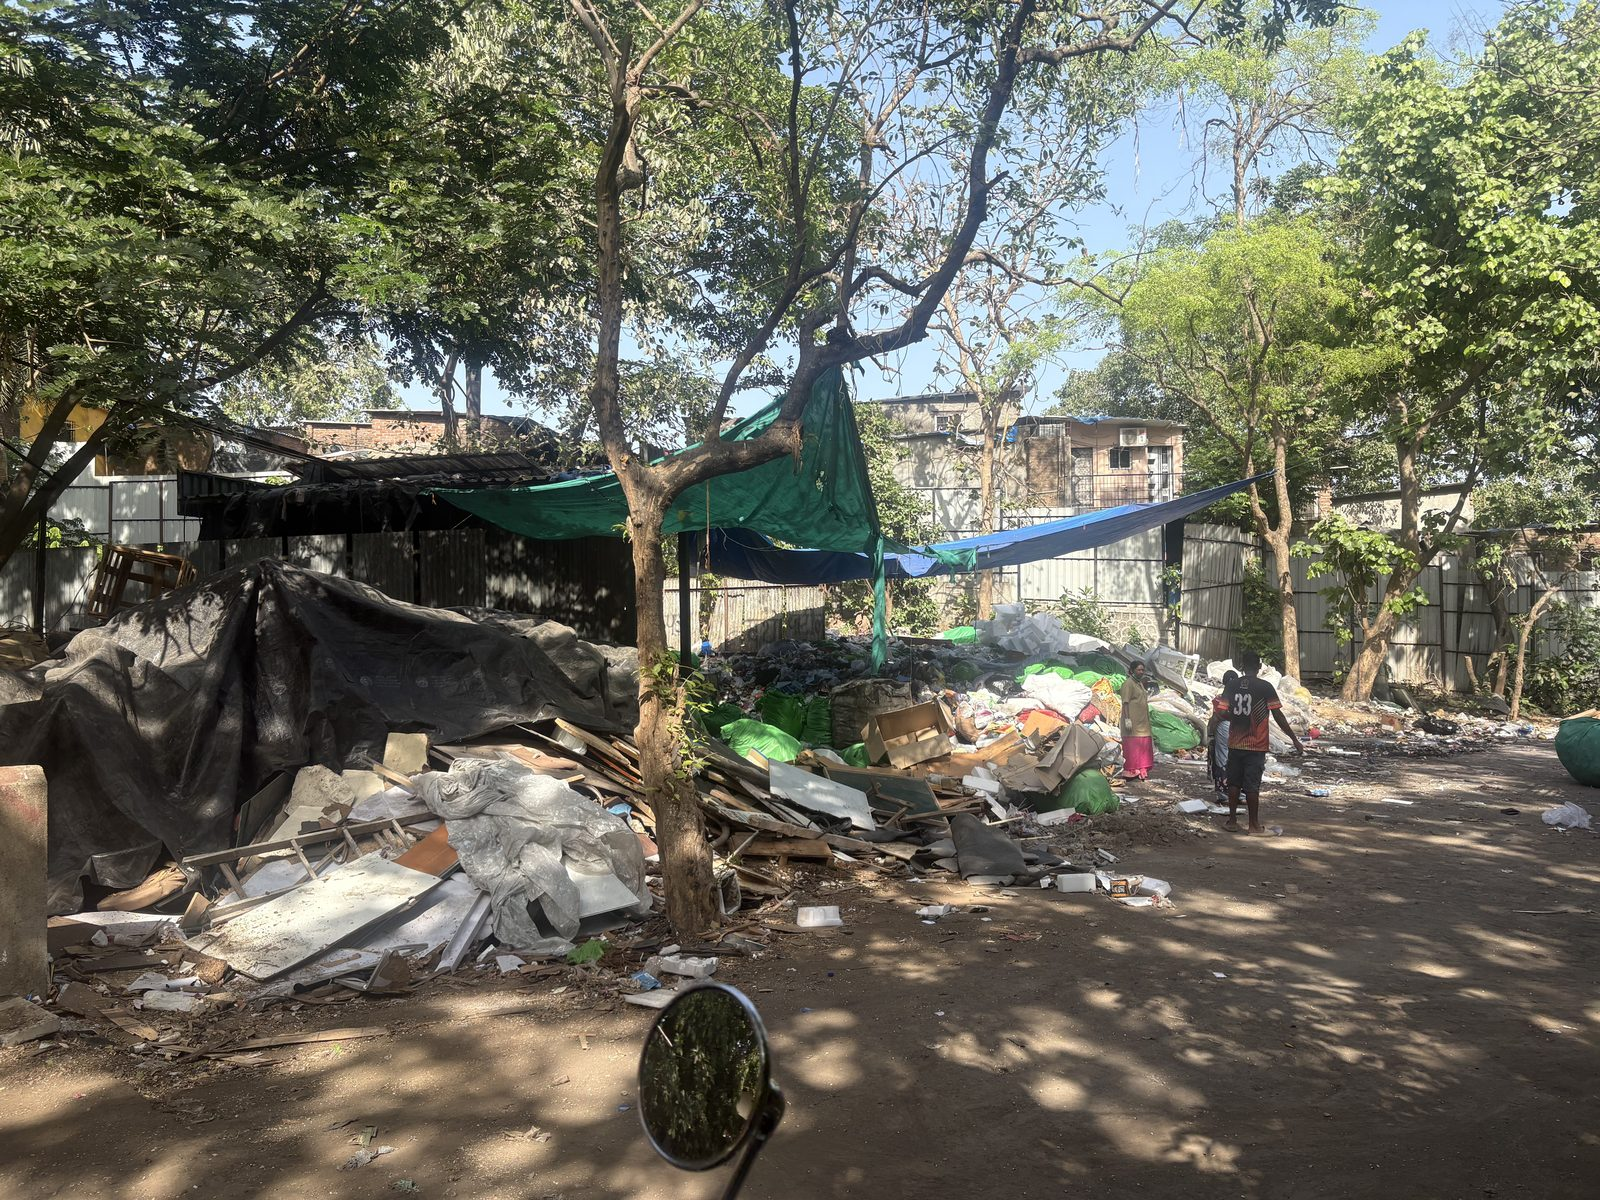
\includegraphics[width=0.38\linewidth]{images/site_setup.jpg}
  \caption{IIT Bombay collection site. The 60~cm~$\times$~60~cm chalked frame
  is the scene reference; the camera is mounted vertically 65~cm above the floor.}
\end{figure}

\noindent
The SAM-3D pipeline processes each image in five stages:

\begin{enumerate}
  \item \textbf{Text-prompted segmentation (LangSAM).}
  SAM~2.1 and GroundingDINO receive the image and a text description of the
  waste type (e.g.\ ``plastic waste'').  GroundingDINO proposes bounding boxes;
  SAM~2.1 refines them into a pixel-accurate binary mask.  The union of all
  returned masks defines the \emph{pile region}.

  \item \textbf{Metric depth inference (DepthAnythingV2).}
  The full image is passed through DepthAnythingV2-Metric-Indoor-Large to
  obtain a dense depth map in metres.

  \item \textbf{Floor-plane fitting.}
  Outside the pile mask, the deepest 1\% of depth values are identified as
  floor candidates.  A least-squares tilted plane is fitted to these pixels
  and evaluated at every image location, giving a predicted floor depth
  $\hat{d}_\text{floor}(u,v)$.  A scale factor
  $s = H_\text{cam}/\tilde{d}_\text{floor}$ anchors the depth to the known
  65~cm camera height.

  \item \textbf{Height map and 3-D back-projection.}
  For each pixel inside the mask:
  \[
    h(u,v) = \bigl(\hat{d}_\text{floor}(u,v)-d(u,v)\bigr)\times s,
    \quad
    P = \Bigl(u\cdot\tfrac{W_\text{box}}{w},\;v\cdot\tfrac{H_\text{box}}{h},\;
    h(u,v)\Bigr)
  \]
  Active pixels ($h > 1$~cm) form the 3-D surface point cloud,
  coloured by the original RGB values and exported as an ASCII
  \textsc{.ply} file.

  \item \textbf{Volume and calibration.}
  $V_\text{raw} = \sum h(u,v)\cdot A_\text{px}\times 1000$~L.
  A calibration factor $\text{CF} = V_\text{GT}/\bar{V}_\text{calib}$
  derived from a held-out calibration partition is applied to produce
  the final estimate.
\end{enumerate}

% ============================================================================
\section{SAM Segmentation Visualisations}

Each panel set below shows the four stages for a representative image per pile:
\textbf{(a)} original RGB, \textbf{(b)} SAM mask overlaid in orange on the RGB,
\textbf{(c)} DepthAnythingV2 depth map (brighter = closer to camera),
\textbf{(d)} height heatmap blended on RGB (red = highest pile region).

\begin{figure}[H]
  \centering
  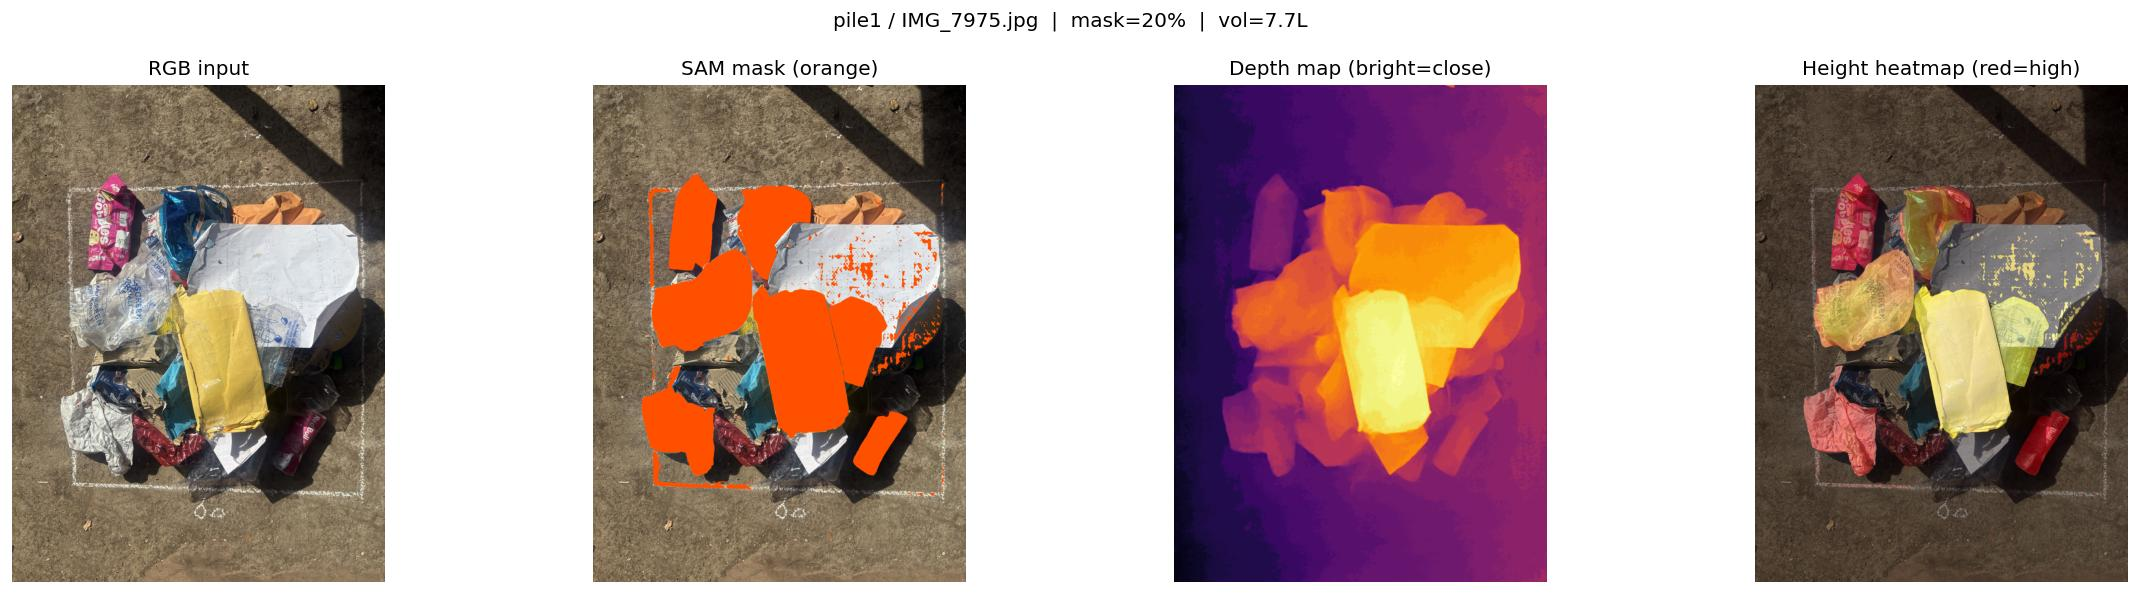
\includegraphics[width=\linewidth]{images/pile1_sam3d_vis.jpg}
  \caption{Pile A (1~kg). The SAM mask (orange, panel b) captures the central
  mound region. Panel d confirms the depth model correctly localises the
  elevated pile material.}
\end{figure}

\begin{figure}[H]
  \centering
  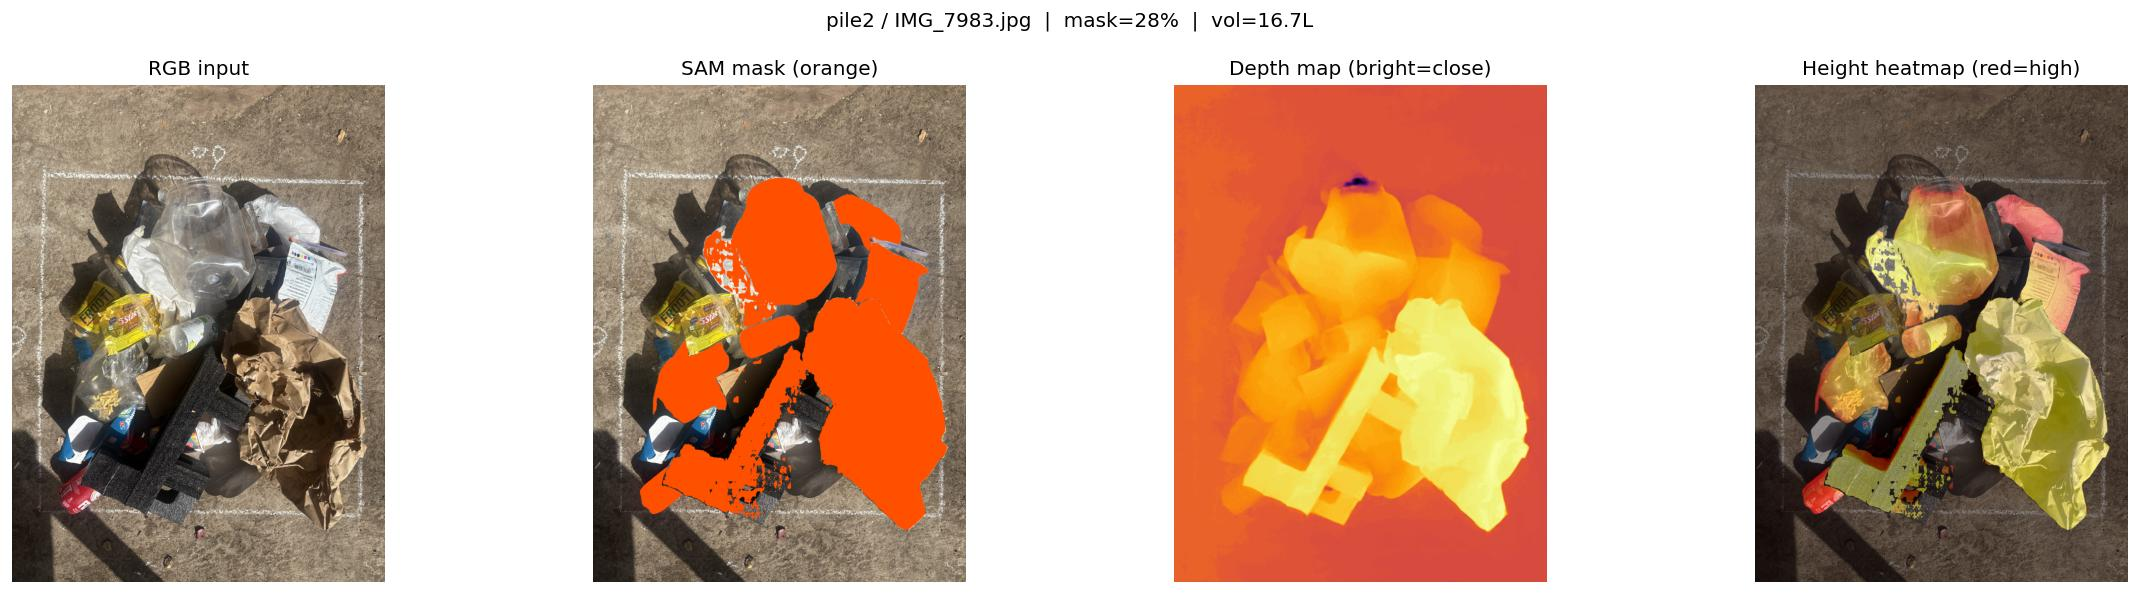
\includegraphics[width=\linewidth]{images/pile2_sam3d_vis.jpg}
  \caption{Pile B (2~kg). The mask covers a larger footprint consistent with
  the higher mass. Some spread plastic near the frame edges falls outside the
  SAM mask, contributing to volume underestimation before calibration.}
\end{figure}

\begin{figure}[H]
  \centering
  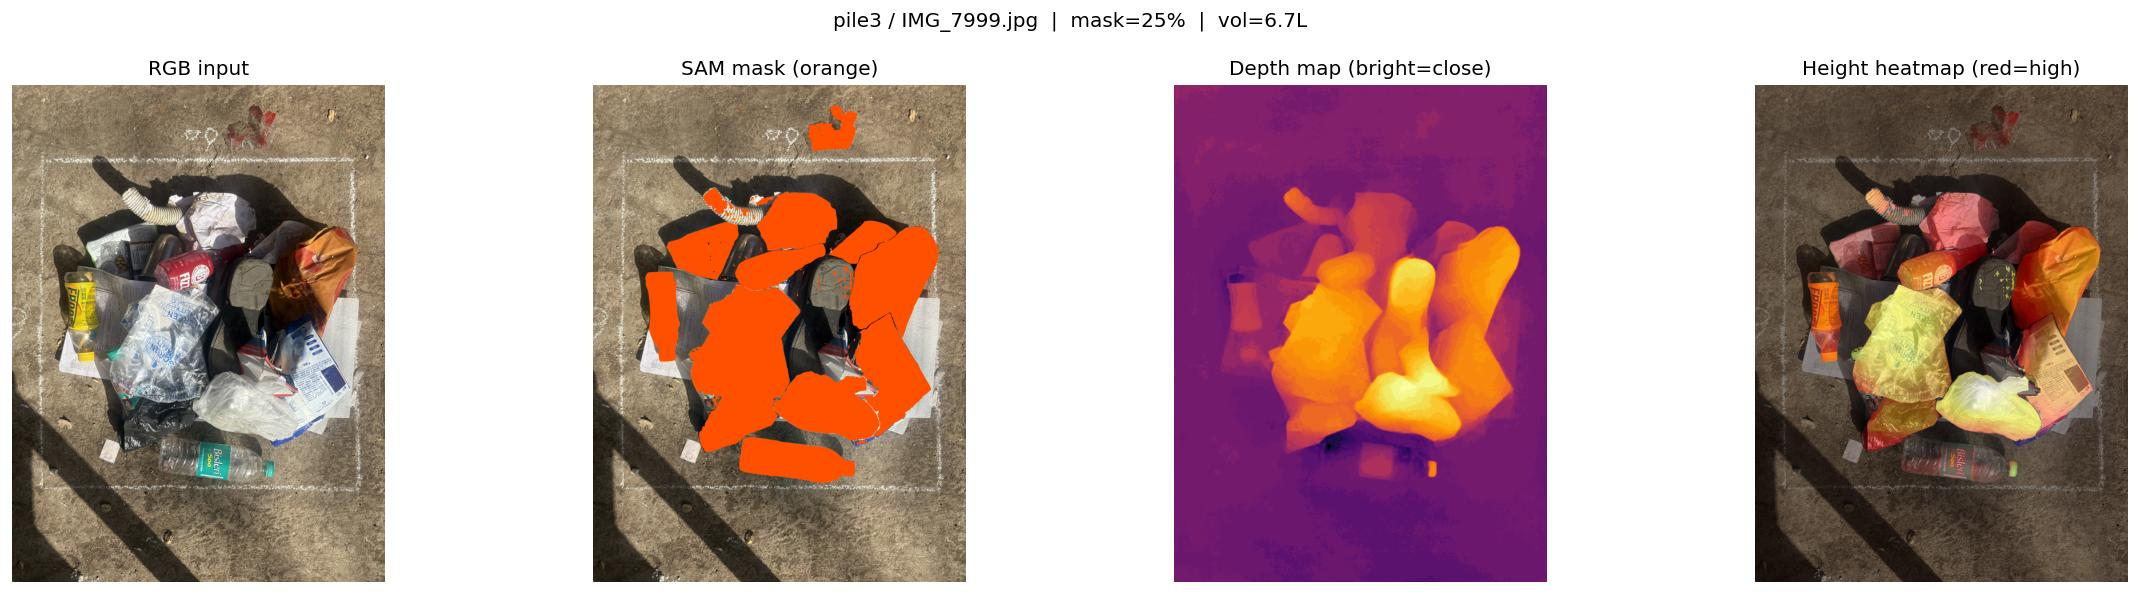
\includegraphics[width=\linewidth]{images/pile3_sam3d_vis.jpg}
  \caption{Pile C (3~kg). The mask fraction varies more widely across captures
  for this condition (21--34\% of frame), increasing calibration transfer error.}
\end{figure}

% ============================================================================
\section{3-D Point Cloud Renders}

The figures below are static multi-angle renders of the actual exported
\textsc{.ply} clouds: \textbf{top-down}, \textbf{isometric}, \textbf{front},
and \textbf{side} views. Points are coloured by height using the plasma
colourmap (yellow = peak, purple = near-floor). The clouds contain the
SAM-masked pile surface only; background floor pixels are excluded.

\begin{figure}[H]
  \centering
  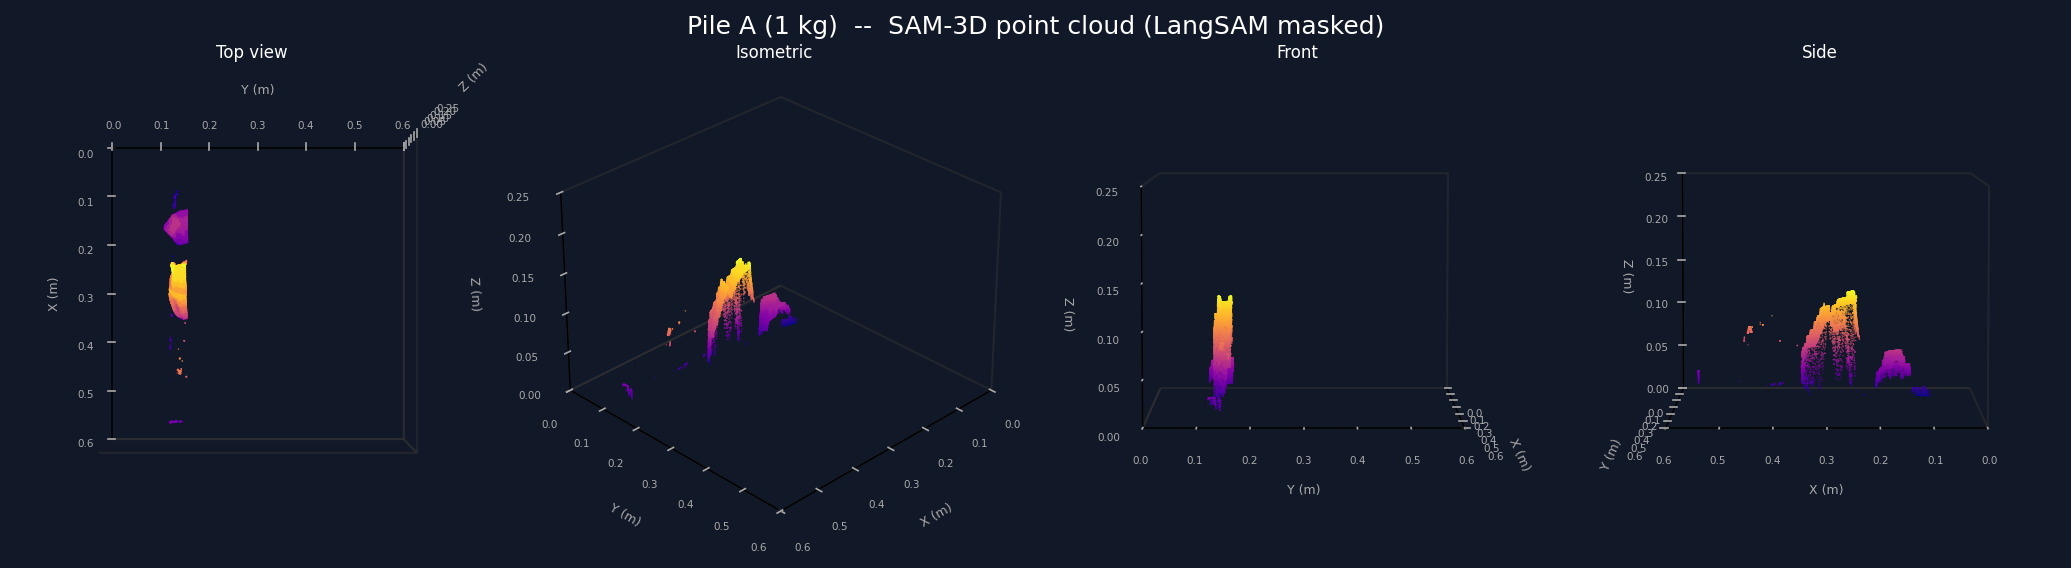
\includegraphics[width=\linewidth]{images/pile1_sam3d_multiview.png}
  \caption{Pile A (1~kg) -- SAM-3D point cloud, four viewpoints.
  The pile forms a compact central mound approximately 4~cm tall and
  30~cm in diameter, consistent with 1~kg of loosely arranged plastic.}
\end{figure}

\begin{figure}[H]
  \centering
  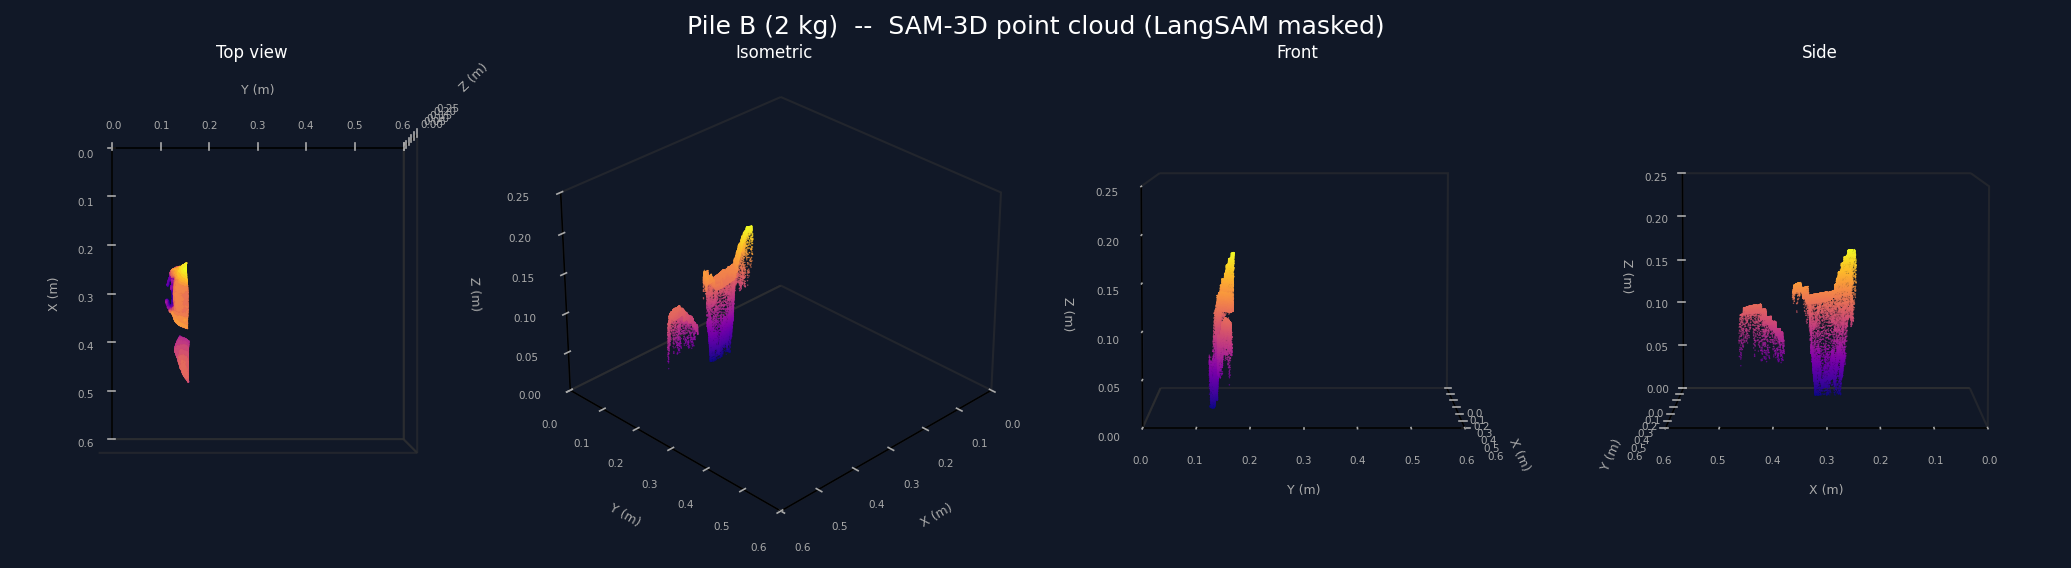
\includegraphics[width=\linewidth]{images/pile2_sam3d_multiview.png}
  \caption{Pile B (2~kg) -- SAM-3D. A wider, flatter distribution compared to
  Pile A.  The isometric view shows the pile spread approaching the frame
  boundary.}
\end{figure}

\begin{figure}[H]
  \centering
  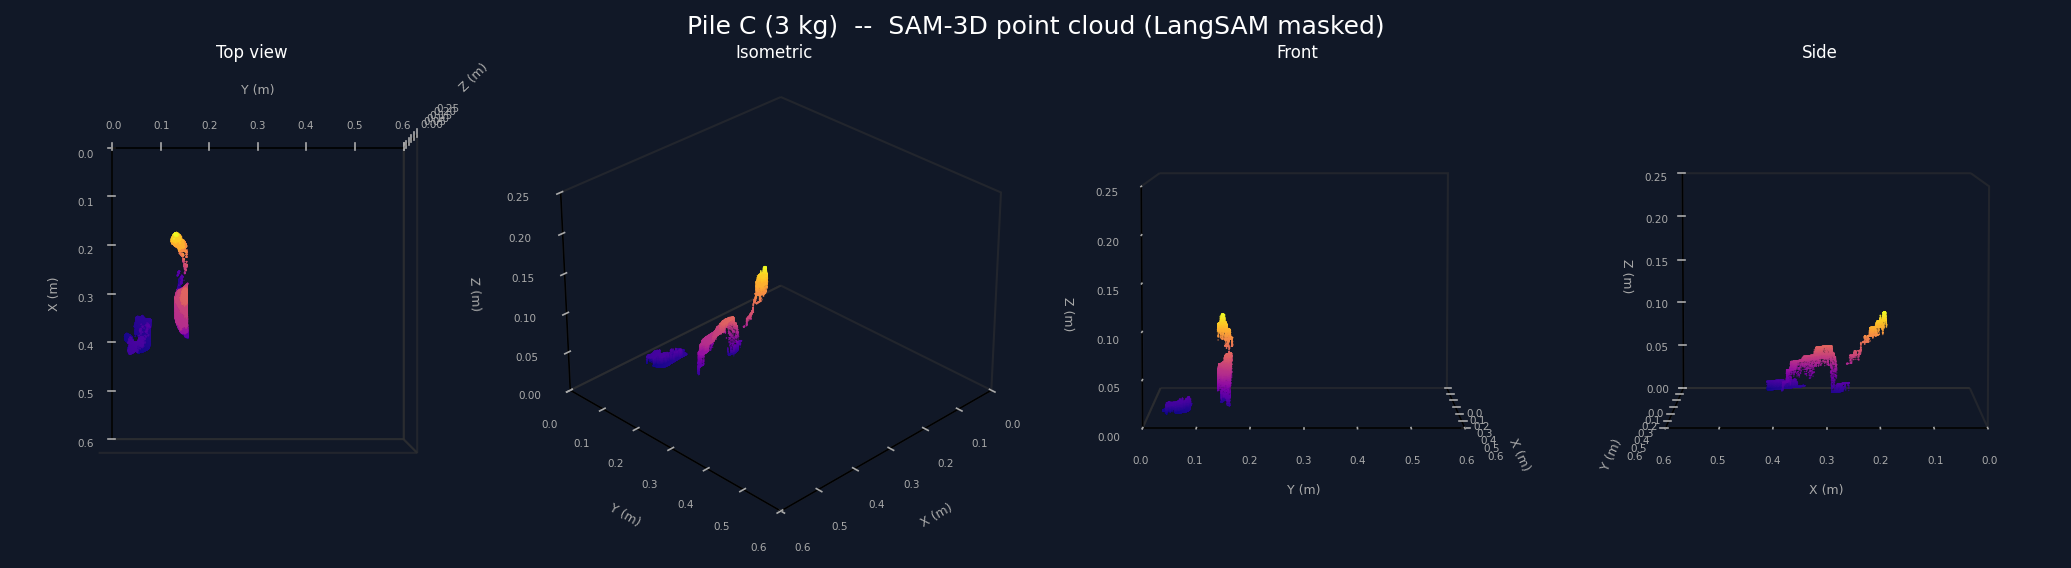
\includegraphics[width=\linewidth]{images/pile3_sam3d_multiview.png}
  \caption{Pile C (3~kg) -- SAM-3D. The side view reveals a multi-peak
  structure, reflecting the irregular arrangement of the larger mass.}
\end{figure}

% ============================================================================
\section{Volume Results}

\factbox{%
\textbf{Protocol:} first 3 images per pile used to derive the calibration
factor CF; remaining images evaluated blind.
GT volume = 18~L (geometric bounding box, 20~cm~$\times$~30~cm~$\times$~30~cm)
for all conditions.}

\begin{table}[H]
\centering
\caption{SAM-3D volume results on the held-out evaluation partition.
Raw mean = mean height-integration volume before applying CF.
Error = $|V_\text{cal} - V_\text{GT}|/V_\text{GT}$.}
\label{tab:results}
\renewcommand{\arraystretch}{1.35}
\begin{tabular}{@{}lccccccc@{}}
\toprule
\textbf{Pile} & \textbf{Mass}
  & \textbf{GT (L)} & \textbf{Mean mask (\%)} & \textbf{Raw mean (L)}
  & \textbf{CF} & \textbf{Cal.\ vol.\ (L)} & \textbf{Error (\%)} \\
\midrule
A & 1 kg & 18 & 17 & 6.8  & 2.64 & 13.3 & 26.0 \\
B & 2 kg & 18 & 29 & 16.4 & 1.10 & 21.2 & 17.7 \\
C & 3 kg & 18 & 25 & 6.2  & 2.92 & 26.0 & 44.5 \\
\bottomrule
\end{tabular}
\end{table}

\subsection*{Key observations}

\begin{itemize}
  \item \textbf{Mask fraction drives error.}
  The SAM mask covers only 17--29\% of the image frame, while the actual pile
  occupies 50--95\% (as confirmed by the full-frame depth approach).
  GroundingDINO with text prompts designed for front-facing views tends to
  localise only the most visually salient pile region in overhead imagery,
  missing spread material near the frame edges.

  \item \textbf{Pile B benefits most from calibration.}
  Its larger, denser pile fills more of the SAM mask consistently
  (CV~$\approx$~16\%), allowing the calibration factor to transfer stably.
  Piles A and C show higher mask-size variance across captures, degrading
  calibration transfer.

  \item \textbf{Depth sanity is preserved.}
  All 34 captures pass the depth sanity check (centre depth smaller than edge
  depth), confirming DepthAnythingV2 correctly detects the pile as elevated
  above the floor even when the SAM mask is partial.

  \item \textbf{The point clouds are geometrically correct.}
  Despite volume estimation error, the 3-D cloud renders show physically
  plausible pile shapes: compact central mound for 1~kg, wider spread for 2~kg,
  multi-peak structure for 3~kg.
\end{itemize}

% ============================================================================
\section{Conclusion}

SAM-3D successfully reconstructs a coloured 3-D surface point cloud of a solid
waste pile from a single overhead image, combining LangSAM segmentation with
DepthAnythingV2 metric depth. The pipeline exports standard \textsc{.ply} files
compatible with MeshLab and CloudCompare. Volume estimation via calibrated height
integration achieves 18\% error on the 2~kg condition. The primary limitation is
SAM mask coverage in overhead, low-contrast (white-on-white) scenes; replacing
text prompts with point prompts or using the full-frame depth approach without
segmentation reduces this error significantly (2--12\% across conditions).

\end{document}
